% chopout for NIPS 2018 workshop on Compact Deep Neural Networks with industrial applications

\documentclass{article}

    % if you need to pass options to natbib, use, e.g.:
    % \PassOptionsToPackage{numbers, compress}{natbib}
    % before loading nips_2018
        
    % ready for submission
    \usepackage{nips_2018}

    % to compile a preprint version, e.g., for submission to arXiv, add
    % add the [preprint] option:
    % \usepackage[preprint]{nips_2018}
    
    % to compile a camera-ready version, add the [final] option, e.g.:
    % \usepackage[final]{nips_2018}
    
    % to avoid loading the natbib package, add option nonatbib:
    % \usepackage[nonatbib]{nips_2018}

    \usepackage[utf8]{inputenc} % allow utf-8 input
    \usepackage[T1]{fontenc}    % use 8-bit T1 fonts
    \usepackage{hyperref}       % hyperlinks
    \usepackage{url}            % simple URL typesetting
    \usepackage{booktabs}       % professional-quality tables
    \usepackage{amsfonts}       % blackboard math symbols
    \usepackage{nicefrac}       % compact symbols for 1/2, etc.
    \usepackage{microtype}      % microtypography
    \usepackage{amsmath}
    \usepackage{amsthm}
    \usepackage{graphicx}
    \usepackage{float}    
    \usepackage{wrapfig}

    \newtheorem{theorem}{Theorem}   
    \newtheorem{lemma}{Lemma} 

    \newcommand{\maximize}{\mathop{\rm maximize}\limits}
    \newcommand{\minimize}{\mathop{\rm minimize}\limits}
    \newcommand{\argmax}{\mathop{\rm arg~max}\limits}
    \newcommand{\argmin}{\mathop{\rm arg~min}\limits}

    
    \title{Chopout: A Simple Way to Train Variable Sized Neural Networks at Once}
 
    % The \author macro works with any number of authors. There are two
    % commands used to separate the names and addresses of multiple
    % authors: \And and \AND.
    %
    % Using \And between authors leaves it to LaTeX to determine where to
    % break the lines. Using \AND forces a line break at that point. So,
    % if LaTeX puts 3 of 4 authors names on the first line, and the last
    % on the second line, try using \AND instead of \And before the third
    % author name.
    
    \author{
      Tatsuya Shirakawa \\
      ABEJA, Inc. \\
      \texttt{tatsuya@abejainc.com}
      %% examples of more authors
      %% \And
      %% Coauthor \\
      %% Affiliation \\
      %% Address \\
      %% \texttt{email} \\
      %% \AND
      %% Coauthor \\
      %% Affiliation \\
      %% Address \\
      %% \texttt{email} \\
      %% \And
      %% Coauthor \\
      %% Affiliation \\
      %% Address \\
      %% \texttt{email} \\
      %% \And
      %% Coauthor \\
      %% Affiliation \\
      %% Address \\
      %% \texttt{email} \\
    }
    
    \begin{document}
    % \nipsfinalcopy is no longer used
    
    \maketitle
    
    \begin{abstract}
      Large deep neural networks require huge memory to run and their running speed is sometimes too slow for real applications. Therefore network size reduction with keeping accuracy is crucial for practical applications. We present a novel neural network operator, \textit{chopout}, with which neural networks are trained, even in a single training process, so as to truncated sub-networks perform as well as possible. \textit{Chopout} is easy to implement and integrate into most type of existing neural networks. Furthermore it enables to reduce network size even after training just by truncating layers. We prove some theoretical aspects of \textit{chopout} and show its effectiveness through several experiments.
    \end{abstract}
    
    % =========================================================
    \section{Introduction}
    % =========================================================
    
    % - deep leraningはデータ・ドリブンなデータサイエンスにとって必要不可欠な道具になった。
    % - 大きさやあアーキテクチャの異なる多種類のモデルが提案されている。
    % - 精度を出すために大きいNNがたくさん提案されている
    %    - ILSVRCの優勝モデル達
    %    - ResNet 1000
    %    - over parametrize
    % - over parametrizedなモデルの方が汎化性能がたかい
    % - 一方で、小さいモデルの方が実行効率がよい。
    %    - SqueezeNet, shuffle net, mobilenet v1/v2
    % - 実行環境によっては大きなメモリを物理的に載せられない
    % - コスト的にも小さいモデルの方がよい
    % - リアルタイムアプリケーションの場合、リアル以上の速度が必要(精度を犠牲にして)
    % - とくにアプリケーションとして動作させるときはコストの面でCPUで動作させることが多く、ネットワークのインファレンスコストはパラメータ数にほぼ比例する。
    % - そのため、精度を落とさずにネットワークのサイズを小さくすることはプラクティカルには非常に重要
    
    Deep neural networks are crucial building blocks for current artificial intelligence (AI)  because of their outstanding performance in accuracy and ease of use. However, such deep neural networks sometimes run too slow and consume too much memories and, therefore, neural networks with less parameters are preferable for applications.
    
    For this end, various parameter size reduction techniques are developed. They includes 
    (1) pruning techniques which aim to prune weights, channels or layers of neural networks (\citet{han2015deep, aghasi2017nettrim, dong2017learning, molchanov2016pruning, li2017pruning, luo2017thinet, ye2018rethinking, liu2017learning, he2017channel}), 
    (2) quantization techniques which aim to quantize weights of neural networks into $\{+1, -1\}$ or lower precision floating points (e.g. fp16) (\citet{han2015learning, courbariaux2015binaryconnect, rastegari2016xnor, zhou2016dorefa, zhu2016trained,  wu2016quantized, hubara2017quantized}), 
    (3) decomposition techniques which aim to decompose weights with combinations of smaller components (e.g. SVD) (\citet{denton2014exploiting, jaderberg2014speeding, lebedev2014speeding, yang2015deep, novikov2015tensorizing}), 
    (4) distillation techniques which aim to train smaller neural networks (student networks) to mimic trained larger neural networks (teacher networks) (\citet{hinton2015distilling, mishra2017apprentice, polino2018model}) and 
    (5) techniques which aim to design more compact but accurate neural networks (\citet{iandola2016squeezenet, howard2017mobilenet, sandler2018mobilenetv2, zhang2017shufflenet}).

    These techniques sometimes can achieve remarkable parameter reduction without too much accuracy decrease. However some of them have limitations of network architectures, are hard to implement using modern deep learning frameworks such as TensorFlow (\citet{abadi2016tensorflow}), Pytorch (\citet{paszke2017automatic}), or MxNet (\citet{chen2015mxnet}) or require model specific adaptations.

    In this research, we proposed a novel stochastic operator \textit{chopout} which is similar to \textit{dropout} (\citet{srivastava2014dropout}) but randomly truncate latter dimensions/channels of layers in neural networks, with which deep neural networks are trained so that their truncated sub-networks also perform well. 

    %Our main contribution in this research is as follows:
    %\begin{itemize} 
    %  \item we provide a novel operator \textit{chopout} which performs dynamic network reduction in training and enhance the accuracy of their truncated sub-networks as well as possible,
    %  \item we prove that training linear autoencoders with \textit{chopout} is equivalent to computing sigular value decomposition of data matrix
    %  \item and we run experiments and show that truncated sub networks perform well
    %\end{itemize}
    
    % =========================================================
    \section{Method}
    % =========================================================
    \label{sec:method}
    
    % ---------------------------------------------------------
    \subsection{Chopout in 1D case}
    % --------------------------------------------------------
    \label{subsec:chopout-1d}
    
    \begin{figure}[tbp]
    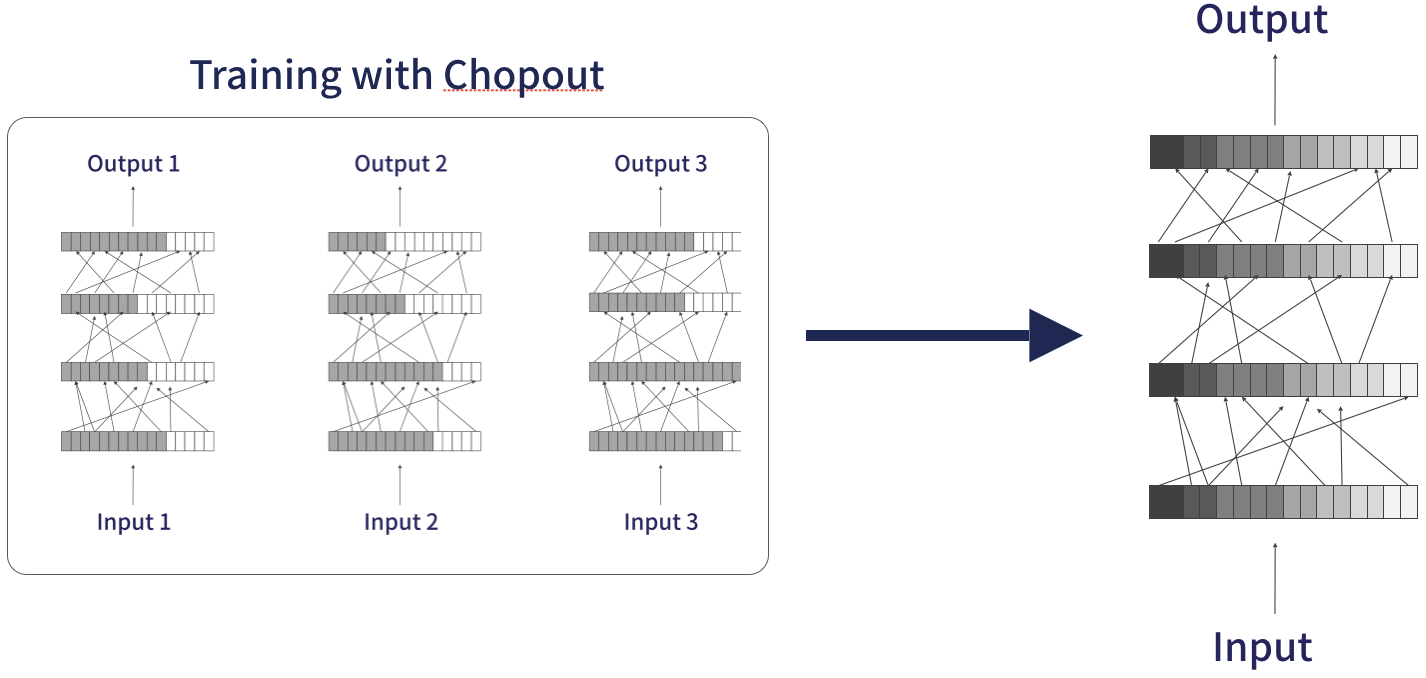
\includegraphics[width=0.7\hsize]{chopout.png}
    \caption{\textit{Chopout} randomly zeros out latter dimensions of vectors in every training iteration, by which important information will be gathered in lower dimensional parts of each layer.}
    \label{chopout}
    \end{figure}
    
    At training time, \textit{Chopout} is defined as a truncation of random-length latter dimensions of vectors as follows:
    \begin{align}
        m \sim P_m = P(\{0, 1, \cdots, d\}), \ \ 
        \mathbf{x} \leftarrow {proj}_m(\mathbf{x}) := (x_1, x_2, ..., x_m, 0, ..., 0) \nonumber
    \end{align}
    where $P_m = P(\{0, 1, \cdots, d\})$ is any discrete distribution over $\{0, 1, \cdots, d\}$ (e.g. uniform distribution), $\mathbf{x} \in \mathbb{R}^d$ is a vector and ${proj}_m(\cdot)$ is a projection to first $m$-th dimensions. 
    \textit{Chopout}'s behavior is similar to \textit{dropout} but, instead of zeroing out random elements in \textit{dropout}, \textit{chopout} zeros out random latter consecutive elements. When back-propagating, the same latter dimensions of gradients are also truncated as well
    \begin{align}
        \mathbf{grad} &\leftarrow {proj}_m(\mathbf{grad}) := ({grad}_1, {grad}_2, ..., {grad}_m, 0, ..., 0) \nonumber
    \end{align}    
    where $\mathbf{grad}$ is a gradient back-propagated from consecutive layers and $m$ is the number drawn in the forward pass. We denote $chopout(\mathbf{x}; P_m)$ or simplty $chopout(\mathbf{x})$ for the above operator.
    
    At test time, \textit{chopout} is defined to behave just same as a identity function, that is, just pass through the input vector without any modification. This definition of \textit{chopout} in prediction mode is contrastive to that of \textit{dropout} because ,ordinarily, in prediction mode, \textit{dropout} is defined as a scaling operator corresponding to its drop-rate.
    
    Training a fully-connected neural network with applying \textit{chopout} can be interpreted as training randomly sampled sub-networks which are obtained by cuttinng out \textit{former parts} of the original fully-connected neural network with sharing parameters.

    % ---------------------------------------------------------
    \subsection{Chopout in the higher dimensional case}
    % ---------------------------------------------------------
    \label{subsec:chopout-nd}
    
    \textit{Chopout} can be easily extended to higher dimensional cases as a random truncation of channels. 
    For example, when applied to a tensor $\mathbf{x} \in 
    \mathbb{R}^{c \times h \times w}$, the forward-propagation of \textit{chopout} is defined as
    \begin{align}
        m \sim P_m = P(\{0, 1, \cdots, c\}), \ \ 
        x_{kij} \leftarrow \begin{cases}
            x_{kij} & (k \leq m) \\
            0 & (otherwise)
            \end{cases} \nonumber
    \end{align}
    where $P(\{0, 1, \cdots, c\}$ is also arbitrary distribution as well (e.g. uniform distribution). We also denote $chopout(\mathbf{x}; P_m)$ or simply $chopout(\mathbf{x})$ for the above operator as well.

    % ---------------------------------------------------------
    \subsection{Linear Autoencoder Case}
    % ---------------------------------------------------------
    \label{subsec:linae}
    
    To clarify the effect of application of \textit{chopout}, we consider a simple case where chopout is applied to linear autoencoder with 1-layer encoder and decoder:
    \begin{align}
        \mathbf{h} = \mathbf{U} \mathbf{x} + \mathbf{b}, \ \ 
        \mathbf{h'} = chopout(\mathbf{h}; P_m), \nonumber \ \
        \mathbf{y} = f(\mathbf{x}; \Theta) := \mathbf{V} \mathbf{h} + \mathbf{c} \nonumber
    \end{align}
    where $\mathbf{x},\mathbf{h}, \mathbf{y} \in \mathbb{R}^d$ are $d$-dimensional input, hidden and output vectors respectively. $P_m$ is a distribution over $\{0, 1, \cdots, d\}$. $\mathbf{U}, \mathbf{V} \in \mathbb{R}^{d \times d}$ are weight matrices, $\mathbf{b}, \mathbf{c} \in \mathbb{R}^d$ are bias vectors and $\Theta = (\mathbf{U}, \mathbf{V}, \mathbf{b}, \mathbf{c})$. We denote the above stochastic reconstruction as $f(\mathbf{x}; \mathbf{\Theta})$. The loss function of this linear autoencoder is mean squared error over training samples $\{\mathbf{x}_1, \mathbf{x}_2, \cdots, \mathbf{x}_n\}$
    \begin{align}
        \minimize_{\Theta} \ \  
        \frac{1}{2n} \sum_{i=1}^n \mathbb{E}_{f} \Vert \mathbf{x}_i - f(\mathbf{x}_i; \Theta) \Vert^2
        = \frac{1}{2n} \sum_{i=1}^n \mathbb{E}_{m \sim P_m} \Vert \mathbf{x}_i - \left( \mathbf{V} \mathbf{I}_m \left( \left( \mathbf{U} \mathbf{x}_i + \mathbf{b} \right) + \mathbf{c} \right) \right) \Vert^2 \label{eq:linear_ae}
    \end{align}
    where $\mathbf{I}_m = diag(1, 1, \cdots, 1, 0, \cdots, 0)$ is a diagonal matrix whose first $m$-th diagonals are one and others are zero. This linear AE optimizaation provably turn to be equivalent to solvoing singular value decomposition (SVD) of data matrix $\mathbf{X} = (\mathbf{x}_1, \mathbf{x}_2, \cdots, \mathbf{x}_n)$ ignoring scaling.

    \begin{theorem}
      \label{th:svd}
      If singular values of $\bar{\mathbf{X}} = \mathbf{P}^T \mathbf{\Sigma} \mathbf{Q}$ are all different, non zero $\sigma_1 > \sigma_2 > \cdots > \sigma_n \geq 0$ and $P_m(m) > 0$ for all $m = 1, \cdots, d$, then, minimizers of (\ref{eq:linear_ae}) satisfy $\mathbf{U} = \mathbf{V}^{-1} = \mathbf{D} \mathbf{P}$ for some diagonal invertible matrix $\mathbf{D} \in \mathbb{R}^{d \times d}$.
    \end{theorem}

    % =========================================================    
    \section{Experiments}
    % =========================================================    
    \label{experiments}
    
    We trained the VGG16 network on cifar10 with or without chopout. The result is in 
    
    Throughout each experiments, we apply \textit{chopout}

    % =========================================================    
    \section{Conclusion}
    % =========================================================    
    \label{Discussion}
    We introduced a novel and easy-to-use and easy-to-implement operator \textit{chopout} and showed that, with \textit{chopout}, neural networks become to be accurate even if their intermediate layers are highly truncated. 
    There could be many direction of further research:
    (1) Applying \textit{chopout} to depth direction, that is, training networks by randomly early stopping at intermediate layers, which enhance sufficiently informative features are extracted at as early layers as possible.
    (2) Applying \textit{chopout} to precision direction of floating points, which might enable training of neural networks consistent in precision of floating points.
    (3) Applying reinforcement learning techniques to \textit{chopout} so as to enable to optimally choose truncation ratio after training.
    (4) Reducing accuracy decrease in case of applying chopout
    %\bibliography{references}
    
    %\section*{References}
    
    %\medskip
    
    %\small
        
    \bibliographystyle{plainnat}
    \bibliography{references}
    
    \end{document}